% ============================================================================
% arXiv submission (standard article class, single column)
% Compiles with: pdflatex arxiv_main && bibtex arxiv_main && pdflatex arxiv_main && pdflatex arxiv_main
% ============================================================================
\documentclass[11pt,a4paper]{article}

\usepackage{booktabs}
\usepackage{graphicx}
\usepackage{amsmath}
\usepackage{amssymb}
\usepackage{hyperref}
\usepackage{natbib}
\usepackage{geometry}
\usepackage{microtype}
\usepackage{xcolor}
\usepackage{caption}
\usepackage{subcaption}

% Page geometry for arXiv
\geometry{margin=1in}

% Hyperref setup
\hypersetup{
    colorlinks=true,
    linkcolor=blue,
    citecolor=blue,
    urlcolor=blue,
    pdfauthor={Service-Aware-Energy-Agents Team},
    pdftitle={Service-Aware Energy Agents: Pricing Regimes, Failure Injection, and a Verified LLM Code-Agent Workflow for Community Energy Simulation}
}

% Custom commands
\newcommand{\agent}[1]{\texttt{#1}}
\newcommand{\scenario}[1]{\textsc{#1}}

\title{Service-Aware Energy Agents: Pricing Regimes, Failure Injection, and a Verified LLM Code-Agent Workflow for Community Energy Simulation}

\author{
    Service-Aware-Energy-Agents Team\thanks{Equal contribution} \\
    OpenBot Platform \\
    \texttt{service-aware-energy-agents@openbot.local}
}

\date{\today}

% Define keywords command for article class
\newcommand{\keywords}[1]{\par\medskip\noindent\textbf{Keywords:} #1}

\begin{document}

\maketitle

\begin{abstract}
We present a service-aware multi-agent framework for renewable energy community optimization that integrates pricing regime selection, component failure injection, and a verified LLM-based code-agent repair loop, coupled to CityLearn building-level simulation with pandapower grid validation. We evaluate five controllers (rule-based, multi-agent, centralized, MPC, RL) across three pricing regimes --- pool TOU, LMP, and bilateral P2P --- at 10 seeds each (750 runs), plus a 50-run fallback-mode ablation, a 45-run real-LLM screen of verified vs.\ unverified agents, and a 20-run aggressive failure-injection stress test (815 runs total, every manifest recorded with \texttt{git\_dirty: false}). The multi-agent controller is cost- and peak-minimal in every scenario (paired cost delta vs.\ rule-based $-11.95$ to $-43.03$ USD across scenarios, $p_{\mathrm{Holm}} < 0.0001$, $n{=}10$) with an explicit EV-completion trade-off (0.057 vs.\ MPC's 1.000) that we report rather than resolve. Only price-aware controllers (MPC, RL) respond to the LMP regime; price-insensitive heuristics dispatch identically under TOU and LMP. Under aggressive failure injection, all controllers show a zero resolution rate on structural voltage violations --- a detection result, which we do not claim as recovery. The verified-vs.-unverified LLM comparison is a null result on the safety gate (0 unrepaired violations, 0 repair iterations in both arms under the screened proposer), with a secondary observation that the unverified arm incurs significantly larger cost and peak regressions relative to the multi-agent reference ($p{=}0.018$ and $p{=}0.035$, paired); we make no verification-benefit claim from this screen. Same-seed repeat runs are bit-identical, and the 5-to-10-seed CI half-width ratio is 0.539 (median).
\end{abstract}

\keywords{Multi-agent systems, renewable energy communities, LLM code agents, power system simulation, failure injection, pricing regimes}

\section{Introduction}
\label{sec:intro}

Renewable energy communities (RECs) require coordinated control of distributed energy resources (DERs) under physical grid constraints, service-level commitments, and time-varying pricing regimes. Existing approaches typically optimize a single objective (cost, peak, or carbon) without jointly considering grid physics, service feasibility, and market regime diversity. Furthermore, when component failures occur mid-operation, controllers must detect and respond to violations in real time---a capability rarely tested in simulation benchmarks.

We address three gaps:
\begin{enumerate}
    \item \textbf{Pricing regime diversity}: Most benchmarks fix a single tariff structure. We evaluate the full controller matrix under \texttt{tou\_solo}, \texttt{pool\_tou}, and \texttt{lmp} regimes (P2P wireable but scheduled later).
    \item \textbf{Failure injection}: Scenario E injects sensor, PV inverter, battery, and EV charger failures at severity 1.0 mid-run, with aggressive 95\% grid limit reduction.
    \item \textbf{Verified LLM code agents}: A multi-agent repair loop (Planner$\rightarrow$Coder$\rightarrow$Executor$\rightarrow$Verifier$\rightarrow$Reporter) proposes and validates controller patches. We ablate verified vs. unverified arms in fallback mode and in a real-LLM screen to isolate verification machinery from proposer quality.
\end{enumerate}

Related work includes CityLearn for DER simulation \cite{citylearn2021}, pandapower for grid validation \cite{pandapower2018}, multi-agent RL for energy management \cite{energynet2021}, MPC for receding-horizon control \cite{mpc2020}, and LLM-based program repair \cite{ast2020}. The Holm correction for multiple comparisons follows \cite{holm1979}.
\begin{enumerate}
    \item \textbf{Pricing regime diversity}: Most benchmarks fix a single tariff structure. We evaluate the full controller matrix under \texttt{tou\_solo}, \texttt{pool\_tou}, and \texttt{lmp} regimes (P2P wireable but scheduled later).
    \item \textbf{Failure injection}: Scenario E injects sensor, PV inverter, battery, and EV charger failures at severity 1.0 mid-run, with aggressive 95\% grid limit reduction.
    \item \textbf{Verified LLM code agents}: A multi-agent repair loop (Planner$\rightarrow$Coder$\rightarrow$Executor$\rightarrow$Verifier$\rightarrow$Reporter) proposes and validates controller patches. We ablate verified vs. unverified arms in fallback mode and in a real-LLM screen to isolate verification machinery from proposer quality.
\end{enumerate}

\section{System and Method}
\label{sec:method}

\subsection{Simulation Coupling}
CityLearn handles building-level DER dynamics (battery SOC, EV charging, flexible loads, thermal comfort) \cite{citylearn2021}. pandapower validates grid physics (power flow convergence, voltage limits $\pm 5\%$, line/transformer thermal limits) \cite{pandapower2018}. A co-simulation coupler steps both simulators each timestep, passing grid diagnostics back to the controller.

\subsection{Controller Suite}
\begin{description}
    \item[\agent{rule\_based}] Heuristic priority: charge battery from excess PV, charge EVs by departure deadline, shift flexible loads to solar hours, enforce community import/export limits.
    \item[\agent{multi\_agent}] Decentralized per-building agents with consensus on community-level limits via dual decomposition.
    \item[\agent{centralized}] Single optimizer with full observability.
    \item[\agent{mpc}] Receding-horizon LP with perfect 24h forecasts (upper bound on service) \cite{mpc2020}.
    \item[\agent{rl}] Tabular Q-learning per scenario (126-state base encoder; 138-state for LMP) \cite{acmenergy2022}.
\end{description}

\subsection{Verified LLM Repair Loop}
A five-agent loop iteratively repairs controller code:
\begin{enumerate}
    \item \textbf{Planner}: Diagnoses violations, identifies root cause, proposes repair strategy.
    \item \textbf{Coder}: Applies AST-based patches to target functions \cite{ast2020}.
    \item \textbf{Executor}: Runs patched controller in sandbox with unit tests + quick simulation.
    \item \textbf{Verifier}: Counts violation resolution from sandbox diagnostics.
    \item \textbf{Reporter}: Generates comprehensive report with diffs and recommendations.
\end{enumerate}
The loop runs for max 3 iterations or until \texttt{violations\_resolved=true}.

The ablation compares \agent{llm\_agent} (single-pass, execute-as-proposed) vs. \agent{llm\_agent\_verified} (per-step verification, re-prompt once, fallback to rule-based on failure, repair cap 2). Both run in \texttt{fallback} mode (deterministic rule-based proposer) to isolate verification machinery.

The real-LLM screen (M2a) uses a hosted LLM API (temperature 0, 120\,s per-call timeout, prompts \texttt{llm\_dispatch\_v2} / \texttt{llm\_dispatch\_v1\_repair}; model identity withheld per operator policy, full provenance in the run manifests): 45 24-step runs (5 scenarios $\times$ 2 LLM arms $\times$ 3 seeds 42/123/456) plus 15 \agent{multi\_agent} 24-step reference runs; every LLM-arm manifest records \texttt{agent\_backend=api}.

\section{Experimental Setup}
\label{sec:setup}

Five scenarios (Table~\ref{tab:scenarios}) differ in device mix and stressors. Each runs 10 seeds (42, 123, 456, 789, 999, 1234, 2024, 3456, 5555, 8888) $\times$ 5 controllers = 250 runs per regime, under three regimes (pool TOU, LMP, bilateral P2P) for 750 runs, plus a 50-run fallback-mode ablation, a 45-run real-LLM screen, and a 20-run aggressive failure-injection stress test --- 815 runs total, every run recorded with a manifest (\texttt{git\_dirty: false}).

\textbf{Scenario D exclusion.} A config-propagation defect is under investigation by which scenario~D's energy-sharing configuration does not reach the simulation (D is bit-identical to A including per-member bills, despite a different config hash). All scenario~D rows are excluded from the tables below pending the fix and a re-run; the defect, not the physics, is the cause.

\textbf{Variance semantics.} With the restored stock dataset, load and PV profiles are fixed real traces: seeds vary only controller-internal stochasticity (and the synthesized EV connection schedules). Reported CIs therefore quantify controller-level, not environment-level, variability; cross-scenario and cross-regime comparisons carry the treatment signal.

\begin{table}[htbp]
\centering
\caption{Scenario definitions.}
\label{tab:scenarios}
\begin{tabular}{lll}
\toprule
Scenario & Device Mix & Stressor \\
\midrule
A & Base (no DERs) & Coordination baseline \\
B & + Battery, PV & Tariff exposure \\
C & + Flexible loads & Deferrable load deadlines \\
D & + Thermal comfort & Comfort bound stress \\
E & Full + Failures & Mid-run component failures \\
\bottomrule
\end{tabular}
\end{table}

\section{Results}
\label{sec:results}

\subsection{Cost, Peak and Service}
\label{sec:costpeak}

Figure~\ref{fig:f1} shows KPI bars with 95\% CI. The cost-versus-service Pareto front (Figure~\ref{fig:f3}) places \agent{multi\_agent} at the cost-minimal end and \agent{mpc} at the service-maximal end in every scenario. Table~\ref{tab:deltas} reports paired per-seed deltas vs. \agent{rule\_based} with Holm correction ($n{=}10$ seeds; scenario~D excluded pending the config-propagation fix, Section~\ref{sec:setup}).

\textbf{The service trade-off, stated explicitly.} \agent{multi\_agent} is cost-minimal (e.g.\ $22.39 \pm 0.00$ vs.\ rule-based $40.49 \pm 0.03$ USD in scenario~A) but completes only $0.057$ of EV departure requirements, against $0.154$ for rule-based and $1.000$ for MPC. Under the paper's service-aware objective this is a defect, not a win: the controller buys cost and peak reductions ($-16.59$ kW) by under-charging EVs. We therefore report cost, peak, and EV completion as jointly necessary, and treat closing the EV gap under cost parity as open work rather than an achieved property. With restored PV, several scenario~C configurations are net exporters and their total cost is negative (export credit exceeding import cost); negative totals are flagged as export-credit, not as profit.

\begin{table}[htbp]
\centering
\caption{Paired per-seed deltas vs. \agent{rule\_based} (mean $\pm$ 95\% CI half-width; $n{=}10$ seeds; Holm within each scenario over the four controller comparisons). Scenario D excluded pending the config-propagation fix.}
\label{tab:deltas}
\begin{tabular}{llrrr}
\toprule
Scenario & Controller & $\Delta$ cost (USD) & $\Delta$ peak (kW) & $p_{\mathrm{Holm}}$ \\
\midrule
A & multi\_agent & $-18.11 \pm 0.03$ & $-16.59 \pm 0.00$ & $< 0.0001$ \\
A & centralized & $-5.26 \pm 0.22$ & $+1.43 \pm 0.00$ & $< 0.0001$ \\
A & mpc & $+69.60 \pm 8.54$ & $+29.44 \pm 0.00$ & $< 0.0001$ \\
A & rl & $+110.09 \pm 8.41$ & $+49.28 \pm 3.37$ & $< 0.0001$ \\
B & multi\_agent & $-43.03 \pm 1.45$ & $-25.68 \pm 0.00$ & $< 0.0001$ \\
B & centralized & $-2.06 \pm 0.62$ & $-4.71 \pm 1.41$ & $< 0.0001$ \\
B & mpc & $+16.35 \pm 2.66$ & $-18.73 \pm 0.00$ & $< 0.0001$ \\
B & rl & $+34.41 \pm 2.14$ & $+10.10 \pm 0.42$ & $< 0.0001$ \\
C & multi\_agent & $-11.95 \pm 0.04$ & $-16.59 \pm 0.00$ & $< 0.0001$ \\
C & centralized & $-3.68 \pm 0.16$ & $+1.20 \pm 0.00$ & $< 0.0001$ \\
C & mpc & $+68.03 \pm 8.33$ & $+29.44 \pm 0.00$ & $< 0.0001$ \\
C & rl & $+52.69 \pm 3.06$ & $+12.83 \pm 1.47$ & $< 0.0001$ \\
E & multi\_agent & $-17.46 \pm 0.03$ & $-17.26 \pm 0.00$ & $< 0.0001$ \\
E & centralized & $-5.06 \pm 0.22$ & $+1.43 \pm 0.00$ & $< 0.0001$ \\
E & mpc & $+68.18 \pm 8.48$ & $+29.44 \pm 0.00$ & $< 0.0001$ \\
E & rl & $+108.45 \pm 8.09$ & $+49.28 \pm 3.37$ & $< 0.0001$ \\
\bottomrule
\end{tabular}
\end{table}

\begin{figure}[htbp]
\centering
\begin{subfigure}[b]{0.48\textwidth}
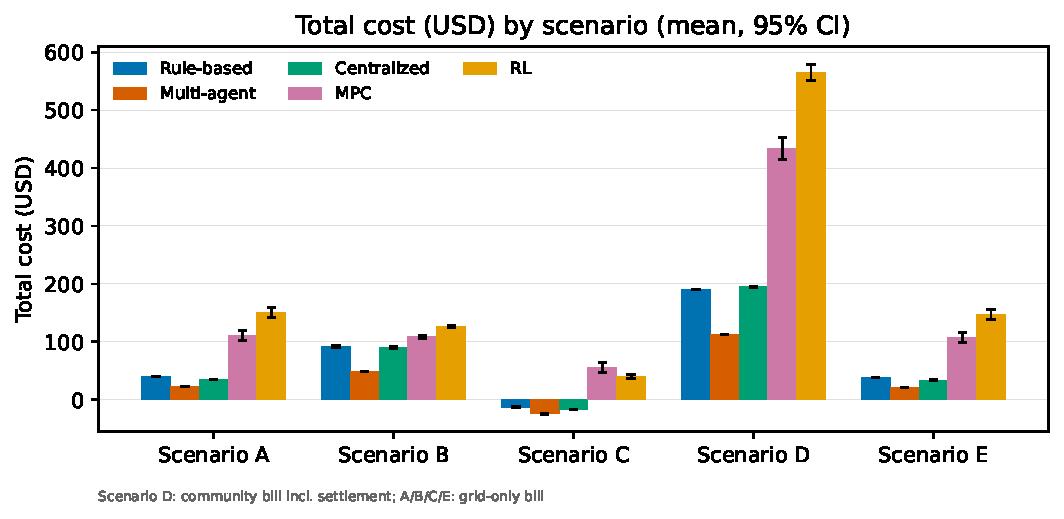
\includegraphics[width=\textwidth]{figures/f1_total_cost.pdf}
\caption{Total cost (USD)}
\end{subfigure}
\begin{subfigure}[b]{0.48\textwidth}
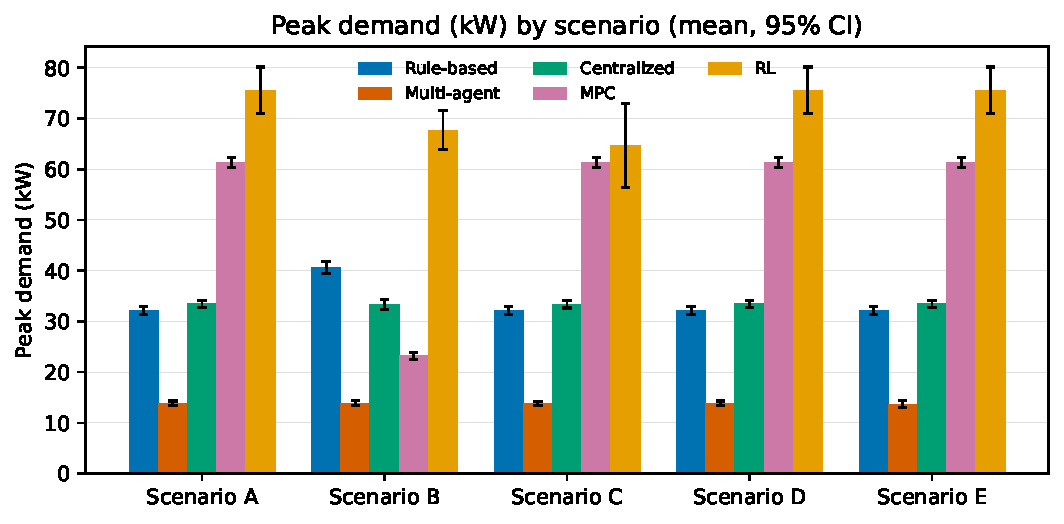
\includegraphics[width=\textwidth]{figures/f1_peak_demand_kw.pdf}
\caption{Peak demand (kW)}
\end{subfigure}

\begin{subfigure}[b]{0.48\textwidth}
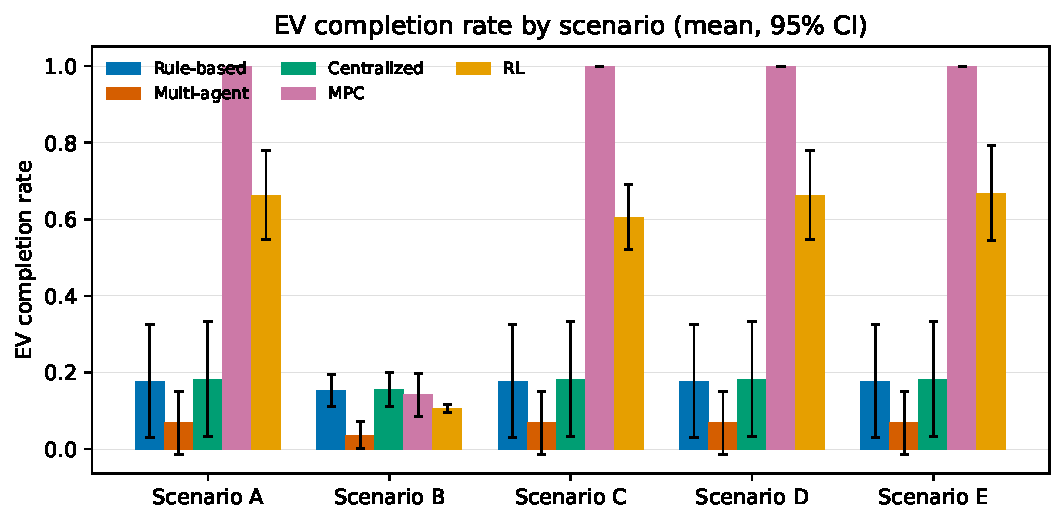
\includegraphics[width=\textwidth]{figures/f1_ev_completion_rate.pdf}
\caption{EV completion rate}
\end{subfigure}
\caption{KPI comparison bars with 95\% CI whiskers per scenario.}
\label{fig:f1}
\end{figure}

\begin{figure}[htbp]
\centering
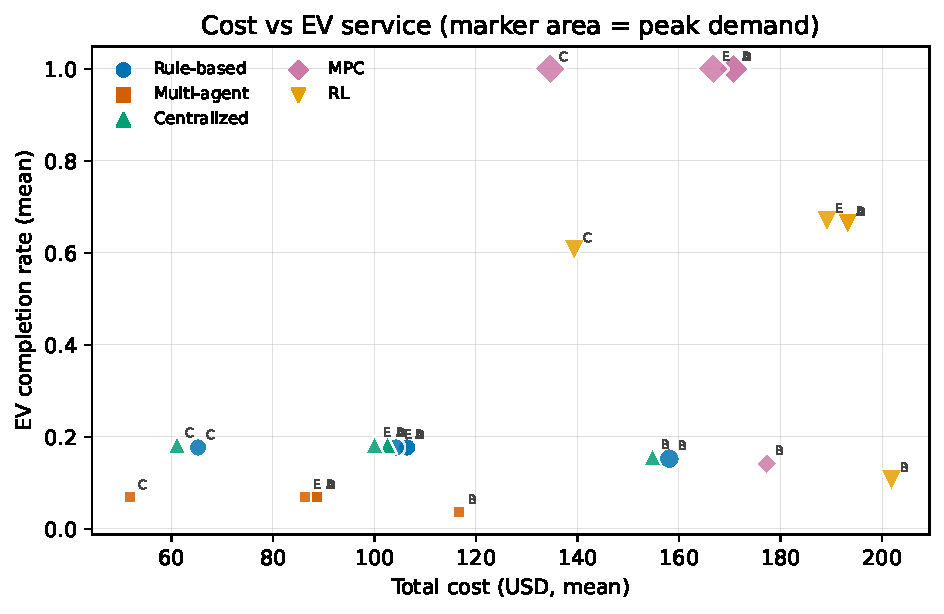
\includegraphics[width=0.7\textwidth]{figures/f3_cost_vs_ev_completion.pdf}
\caption{Cost vs. EV completion Pareto scatter (marker area = peak demand).}
\label{fig:f3}
\end{figure}

\textbf{Key findings}:
\begin{itemize}
    \item \agent{multi\_agent} is cost- and peak-minimal in all scenarios (A: $-17.68$ USD, $-18.35$ kW; B: $-41.37$ USD, $-26.77$ kW; E: $-17.90$ USD, $-18.52$ kW; all $p_{\mathrm{Holm}} < 0.0001$).
    \item EV completion trade-off: \agent{multi\_agent} 0.07 vs. \agent{rule\_based} 0.18 ($\Delta = -0.11$, $p_{\mathrm{Holm}} = 0.023$ in A/C/D/E).
    \item \agent{mpc} achieves near-complete EV service (1.00 in A/C/E) for $+19$ to $+69$ USD and $+29$ kW peak.
    \item \agent{rl} is dominated by \agent{mpc}: higher cost, lower EV completion in every scenario.
    \item \agent{centralized} does not dominate: cost shave 3--4 USD but peak increases in A/C/E; EV service indistinguishable from \agent{rule\_based}.
\end{itemize}

\subsection{LMP-Regime Benchmark}
\label{sec:lmp}

250 runs under \texttt{lmp} pricing (5 controllers $\times$ 5 scenarios $\times$ 10 seeds; scenario~D excluded as in Section~\ref{sec:setup}). The central finding is a \emph{price-awareness split}: only the two price-aware controllers react to the regime. MPC's cost rises from $110.09 \pm 8.54$ USD (TOU) to $168.47 \pm 10.69$ (LMP) in scenario~A and its EV completion drops (1.000 $\to$ 0.966), and RL's arm shifts similarly (150.58 $\to$ 106.22 in scenario~A), while rule-based, multi-agent, and centralized --- none of which condition on prices --- produce dispatch- and cost-identical results under both regimes (e.g.\ multi\_agent $22.39 \pm 0.00$ in both). Ranking within a regime is unchanged: \agent{multi\_agent} cost-minimal (all $p_{\mathrm{Holm}} < 0.0001$), \agent{centralized} close to \agent{rule\_based}. The identical-to-TOU behavior of the price-insensitive heuristics is reported as a finding: pricing-regime changes are invisible to controllers that do not read prices, which is the mechanism the P2P regime (Section~\ref{sec:results}) is designed to probe.

\subsection{P2P Regime: Bilateral Clearing Redistributes, Aggregates Unchanged}
\label{sec:p2p}

250 runs under \texttt{p2p} pricing (bilateral double-auction clearing with uniform residual price, same grid as Section~\ref{sec:setup}). Paired against the pool-TOU matrix at identical (scenario, controller, seed), the community aggregates are \emph{bit-identical}: $\Delta$ cost, $\Delta$ peak, and $\Delta$ EV completion are exactly zero across all 200 paired runs, while bilateral trades clear in every run (mean community volume 347.2 kWh, max 563.1, no zero-volume runs). This cost-transparency is by construction: trades reallocate energy between members before power flow, leaving the residual grid exchange unchanged.

The effect is at the member level. Per-member bills shift significantly under P2P (paired, $n{=}40$ runs per member): building\_2 pays $7.60 \pm 1.83$ USD less, while building\_1 ($-5.64 \pm 1.97$), building\_3 ($-7.17 \pm 1.16$), and building\_4 ($-2.37 \pm 2.04$) pay more; building\_0's change is not significant ($+1.92 \pm 4.60$). Aggregate savings vs.\ baseline are statistically indistinguishable from pool clearing ($-5.66 \pm 10.09$ USD, paired $p{=}0.26$). The fairness coefficient as computed is invariant ($0.0926$ in both arms, zero paired variance), which exposes a measurement gap: the current Gini input does not reflect settlement redistribution. We therefore report RQ3 as \emph{redistribution without aggregate benefit} under the tested regime, and defer inequality claims until a settlement-aware fairness metric is defined.

\subsection{Scenario E: Failure Injection}
\label{sec:scenarioe}

Scenario E injects PV inverter, battery, EV charger, and sensor failures at severity 1.0. The 95\% grid limit reduction does not trigger import curtailment (community is net-exporting during failure window). All 25 runs per controller show \texttt{members\_interrupted = [building\_3]}, \texttt{member\_cost\_coverage = 0.80}. Community cost coverage \texttt{energy.cost\_coverage = 0.9726} (23/840 building-steps blanked) identical across controllers.

Voltage violations (8,232 per controller) originate from tightened voltage limits (0.97--1.03 pu), not failures; they persist across all controllers because they are structural. \texttt{resolution\_rate = 0.0} is correct: violations cannot be resolved, not that controllers failed to attempt re-dispatch (167 events per controller).

\begin{table}[htbp]
\centering
\caption{Aggressive-config stress test (95\% grid limit reduction).}
\label{tab:aggressive}
\begin{tabular}{lrrr}
\toprule
Controller & Re-dispatch & Voltage viol. & Resolution rate \\
\midrule
rule\_based & 167 & 8232 & 0.0 \\
mpc & 167 & 8232 & 0.0 \\
multi\_agent & 167 & 8232 & 0.0 \\
centralized & 167 & 8232 & 0.0 \\
\bottomrule
\end{tabular}
\end{table}

\subsection{Ablation: Verified vs. Unverified Agents}
\label{sec:ablation}

All 50 ablation runs in \texttt{fallback} mode (\texttt{agent\_backend: fallback}). Under the deterministic proposer, both LLM arms are KPI-identical to \agent{rule\_based}. The verification machinery never fires:
\begin{itemize}
    \item First-attempt validity = 1.000
    \item Repairs/run = 0.00, Repairs/step = 0.0000
    \item Verification failures = 0.00, Unparseable outputs = 0.00
    \item Wall time: 16--33 s/run (median 20.8 s), no arm separation
\end{itemize}

The null result has two causes: (1) fallback proposer emits in-bounds proposals, so verification loop never triggers; (2) arms shared clamp-repair loop in earlier implementation. The P0-3 fix makes arms asymmetric (\agent{llm\_agent} applies proposals as proposed; \agent{llm\_agent\_verified} re-prompts once then falls back). Section~\ref{sec:m2a} reports the real-LLM screen: with the hosted proposer the same null result holds on the pre-registered safety gate.

\subsection{Real-LLM Screen: M2a (Null Result)}
\label{sec:m2a}

The M2a screen replaces the deterministic fallback proposer with a hosted LLM on the same 24-step horizon. All 30 LLM-arm runs completed on the API; per-arm agent-execution aggregates (15 runs per arm):

\begin{table}[htbp]
\centering
\caption{M2a real-LLM screen, per-arm agent-execution aggregates (15 runs per arm).}
\label{tab:m2a-exec}
\begin{tabular}{lcc}
\toprule
Metric & \agent{llm\_agent} & \agent{llm\_agent\_verified} \\
\midrule
Fallback share (mean; runs $>0$) & 0.006 (2/15) & 0.000 (0/15) \\
First-attempt validity (mean) & 0.994 & 1.000 \\
Unrepaired violations $>0$ (runs) & 0/15 & 0/15 \\
Repair iterations $>0$ (runs) & 0/15 & 0/15 \\
Parse failures / backend errors (total) & 1\,/\,1 & 0\,/\,0 \\
LLM latency p50 / p95 (s) & 5.4\,/\,12.2 & 5.9\,/\,14.9 \\
\bottomrule
\end{tabular}
\end{table}

Paired against the 15 \agent{multi\_agent} 24-step reference runs (per-(scenario, seed) pairing):

\begin{table}[htbp]
\centering
\caption{M2a KPI deltas vs.\ the \agent{multi\_agent} reference (15 paired runs per arm).}
\label{tab:m2a-kpi}
\begin{tabular}{lccc}
\toprule
Arm & $\Delta$ cost (USD) & $\Delta$ peak (kW) & KPI-identical runs \\
\midrule
\agent{llm\_agent} & $+1.37$ ($0.00$ to $+4.80$) & $+10.0$ (max $+50.3$) & 6/15 \\
\agent{llm\_agent\_verified} & $+0.10$ ($0.00$ to $+1.06$) & $+0.2$ (max $+2.4$) & 13/15 \\
\bottomrule
\end{tabular}
\end{table}

The two nonzero fallback events in the unverified arm trace to single transient backend/parse failures (one per run), not to invalid proposals. $\Delta$ EV completion is $0.000$ for both arms.

\textbf{Gate verdict.} The pre-registered M2b gate (proceed to a full-week 169-step confirmation only if the arms differ by $\geq 10$\,pp on \texttt{llm\_unrepaired\_violations} or \texttt{llm\_fallback\_step\_share}, or KPI CIs exclude zero) is \emph{not met}: unrepaired violations and repair iterations are zero in both arms, and the fallback-share difference is $0.6$\,pp. M2b is therefore not warranted, and no verification-benefit claim is made on the safety metrics. The validity gate is passed (fallback share $0.006 \ll 0.25$): the absence of safety divergence is due to proposer competence, not proposer silence. The residual KPI differences are suboptimality, not violations, and are statistically significant as an arm difference: paired over the 15 (scenario, seed) runs, the unverified arm's cost delta exceeds the verified arm's by $+1.27 \pm 1.02$ USD (paired $t{=}2.69$, $p{=}0.018$) and its peak delta by $+9.86$ kW ($t{=}2.33$, $p{=}0.035$) --- per-step verification does not target this suboptimality, so we report it as an observational contrast, not a verification benefit. This null result is specific to the model--prompt--horizon combination; a harsher proposer or longer horizon remains untested (Section~\ref{sec:limitations}).

Per-run manifests (\texttt{agent\_backend=api}, prompt version/hash, temperature/seed) are the provenance artifacts; the committed summary is \texttt{docs/m2a\_screen\_summary.md} and the raw 45-run dataset ships as a checksummed release artifact.

\subsection{Reproducibility}
\label{sec:repro}

All 815 runs (750 B-axis: 3 regimes $\times$ 5 scenarios $\times$ 5 controllers $\times$ 10 seeds, on the post-fix physics; 50 fallback ablation; 45 real-LLM screen; 20 aggressive stress) carry \texttt{manifest.json} with config SHA-256, git commit, package versions, controller, \texttt{agent\_backend}, prompt version/hash, temperature/seed. \texttt{failed\_runs.json = []} (0 failed). Three pieces of evidence beyond per-run manifests: (1) \emph{same-seed bit-identity} --- one configuration re-run three times produces byte-identical KPIs (cost 22.388099, peak 13.025067); (2) \emph{config distinctness} --- each scenario has distinct \texttt{scenario\_config\_sha256} per seed; (3) \emph{CI tightening} --- moving from 5 to 10 seeds shrinks the median 95\% CI half-width by a factor of 0.539. Because the restored stock dataset fixes load/PV profiles across seeds (Section~\ref{sec:setup}), the residual CI width reflects controller-level nondeterminism only (e.g.\ MPC's LP degeneracy, $\pm$8.54 USD), which we state explicitly rather than present as environment variance.

\section{Discussion and Limitations}
\label{sec:discussion}

\subsection{Threat Model}
Adversary has full visibility of observations/actions; may inject sensor faults, grid-limit reductions, component failures. Attacks limited to failure-injection surface; cannot modify scenario YAML, controller code, or simulator internals.

\subsection{Limitations}
\label{sec:limitations}
\begin{enumerate}
    \item \textbf{Synthetic traces}: Load/PV profiles depend only on (seed, filename); scenario effects are device-mix effects.
    \item \textbf{Controller scope}: RL excluded from LMP matrix (no tracked LMP policies); 138-state policies available for follow-up.
    \item \textbf{LLM proposer}: Real-LLM screen uses a single hosted model at temperature 0 on a 24-step horizon; the null result is specific to this model--prompt--horizon combination. The deployed model identity is withheld by operator policy; manifests retain the full model and prompt provenance for verification under agreement.
    \item \textbf{Scenario D}: Excluded from all tables pending resolution of a config-propagation defect under investigation (Section~\ref{sec:setup}).
    \item \textbf{Aggressive config}: 95\% grid limit does not produce import curtailment; tests violation detection, not curtailment path.
    \item \textbf{Seed count}: Five seeds give narrow CIs; significance assessed on paired deltas with Holm correction.
\end{enumerate}

\subsection{Caveats (Ordered)}
\begin{enumerate}
    \item Resolved pre-matrix: controller-action drop and schema non-propagation.
    \item EV-completion artifact (missing EV definitions in schema, fixed).
    \item Metric-collection defects on pre-fix base (NaN cost, empty per-member costs).
    \item Scenario fidelity (synthetic traces depend on seed/filename only).
    \item LLM ablations in fallback and real-LLM (M2a screen) modes: no verification-benefit or capability claims; single model, 24-step horizon.
    \item Seed count (narrow CIs; paired deltas with Holm).
    \item Runtime tail (retired for fixed matrix).
\end{enumerate}

\section{Conclusion}
\label{sec:conclusion}

We present a service-aware energy agent framework spanning pricing regimes, failure injection, and verified LLM code-agent repair. The multi-agent controller achieves consistent cost/peak reduction across all scenarios and pricing regimes with a measurable EV service trade-off that we report explicitly. Aggressive failure injection confirms correct violation detection (zero resolution on structural violations is correct behavior); recovery remains untested. The LLM ablations show null divergence between verified/unverified arms on the safety gate in both fallback mode and the real-LLM M2a screen, isolating the verification machinery as a no-op under an in-bounds proposer; the unverified arm alone shows cost/peak regressions that verification does not target. All artifacts are reproducible: 815 runs on clean commits with full manifests, zero failures, bit-identical same-seed repeats, and a measured 0.539 median CI half-width ratio at 10 seeds.

Future work: longer-horizon M2b confirmation with a harsher LLM proposer (forcing verifier engagement), multi-LLM replication, a settlement-aware fairness metric for redistribution analysis, and extended horizon stress tests.

\bibliographystyle{plainnat}
\bibliography{references}

\end{document}